\documentclass[12pt,letterpaper]{article}
\usepackage{graphicx,textcomp}
\usepackage{natbib}
\usepackage{setspace}
\usepackage{fullpage}
\usepackage{color}
\usepackage[reqno]{amsmath}
\usepackage{amsthm}
\usepackage{fancyvrb}
\usepackage{amssymb,enumerate}
\usepackage[all]{xy}
\usepackage{endnotes}
\usepackage{lscape}
\newtheorem{com}{Comment}
\usepackage{float}
\usepackage{hyperref}
\newtheorem{lem} {Lemma}
\newtheorem{prop}{Proposition}
\newtheorem{thm}{Theorem}
\newtheorem{defn}{Definition}
\newtheorem{cor}{Corollary}
\newtheorem{obs}{Observation}
\usepackage[compact]{titlesec}
\usepackage{dcolumn}
\usepackage{tikz}
\usetikzlibrary{arrows}
\usepackage{multirow}
\usepackage{xcolor}
\newcolumntype{.}{D{.}{.}{-1}}
\newcolumntype{d}[1]{D{.}{.}{#1}}
\definecolor{light-gray}{gray}{0.65}
\usepackage{url}
\usepackage{listings}
\usepackage{color}

\definecolor{codegreen}{rgb}{0,0.6,0}
\definecolor{codegray}{rgb}{0.5,0.5,0.5}
\definecolor{codepurple}{rgb}{0.58,0,0.82}
\definecolor{backcolour}{rgb}{0.95,0.95,0.92}

\lstdefinestyle{mystyle}{
	backgroundcolor=\color{backcolour},   
	commentstyle=\color{codegreen},
	keywordstyle=\color{magenta},
	numberstyle=\tiny\color{codegray},
	stringstyle=\color{codepurple},
	basicstyle=\footnotesize,
	breakatwhitespace=false,         
	breaklines=true,                 
	captionpos=b,                    
	keepspaces=true,                 
	numbers=left,                    
	numbersep=5pt,                  
	showspaces=false,                
	showstringspaces=false,
	showtabs=false,                  
	tabsize=2
}
\lstset{style=mystyle}
\newcommand{\Sref}[1]{Section~\ref{#1}}
\newtheorem{hyp}{Hypothesis}

\title{Problem Set 2}
\date{Due: October 15, 2023}
\author{Applied Stats/Quant Methods 1}

\begin{document}
	\maketitle
	\section*{Instructions}
\begin{itemize}
	\item Please show your work! You may lose points by simply writing in the answer. If the problem requires you to execute commands in \texttt{R}, please include the code you used to get your answers. Please also include the \texttt{.R} file that contains your code. If you are not sure if work needs to be shown for a particular problem, please ask.
	\item Your homework should be submitted electronically on GitHub.
	\item This problem set is due before 23:59 on Sunday October 15, 2023. No late assignments will be accepted.

\end{itemize}

	
	\vspace{.5cm}
	\section*{Question 1: Political Science}
		\vspace{.25cm}
	The following table was created using the data from a study run in a major Latin American city.\footnote{Fried, Lagunes, and Venkataramani (2010). ``Corruption and Inequality at the Crossroad: A Multimethod Study of Bribery and Discrimination in Latin America. \textit{Latin American Research Review}. 45 (1): 76-97.} As part of the experimental treatment in the study, one employee of the research team was chosen to make illegal left turns across traffic to draw the attention of the police officers on shift. Two employee drivers were upper class, two were lower class drivers, and the identity of the driver was randomly assigned per encounter. The researchers were interested in whether officers were more or less likely to solicit a bribe from drivers depending on their class (officers use phrases like, ``We can solve this the easy way'' to draw a bribe). The table below shows the resulting data.

\newpage
\begin{table}[h!]
	\centering
	\begin{tabular}{l | c c c }
		& Not Stopped & Bribe requested & Stopped/given warning \\
		\\[-1.8ex] 
		\hline \\[-1.8ex]
		Upper class & 14 & 6 & 7 \\
		Lower class & 7 & 7 & 1 \\
		\hline
	\end{tabular}
\end{table}

\begin{enumerate}
	
	\item [(a)]
	Calculate the $\chi^2$ test statistic by hand/manually (even better if you can do "by hand" in \texttt{R}).\\
	\vspace{0cm}
	\subsection*{Answer:}
	H0: Class of drivers has no affect on police soliciting bribes from drivers.
	
	Ha: Class of drivers has an affect on police soliciting from drivers.
	\begin{verbatim}
		#Purely by hand.
		#First calculate the expected frequencies, and then put them into the formula below.
		
		((27/42)*21) = 13.5
		((27/42)*13) = 8.36
		((27/42)*8) = 7.5
		((15/42)*21) = 5.14
		((15/42)*13) = 4.64
		((15/42)*8) = 2.86
		
		{(((14-13.5)^2)/13.5)+
			(((6-8.36)^2)/8.36)+
			(((7-7.5)^2)/7.5)+ 
			(((7-5.14)^2)/5.14)+
			(((7-4.64)^2)/4.64)+   
			(((1-2.86)^2)/2.86)
		} 
		= 3.801141
		
		#By hand, naming all the frequencies to avoid rounding.
		
		F01 <- 14
		F02 <- 6
		F03 <- 7
		F04 <- 7
		F05 <- 7
		F06 <- 1
		
		Fe1 <- ((27/42)*21)
		Fe2 <- ((27/42)*13)
		Fe3 <- ((27/42)*8)
		Fe4 <- ((15/42)*21)
		Fe5 <- ((15/42)*13)
		Fe6 <- ((15/42)*8)
		
		{(((F01-Fe1)^2)/Fe1)+
			(((F02-Fe2)^2)/Fe2)+
			(((F03-Fe3)^2)/Fe3)+
			(((F04-Fe4)^2)/Fe4)+
			(((F05-Fe5)^2)/Fe5)+
			(((F06-Fe6)^2)/Fe6)
		} <- test.result
		= 3.791168
	\end{verbatim}
	
	The purely by hand method gives an answer of 3.801141, and the method where the frequencies are named to avoid rounding gives an answer of 3.791168. The difference between the answers is what would be expected when the rounding of the expected frequencies is taken into consideration.
	
	
	\item [(b)]
	Now calculate the p-value from the test statistic you just created (in \texttt{R}).\footnote{Remember frequency should be $>$ 5 for all cells, but let's calculate the p-value here anyway.}  What do you conclude if $\alpha = 0.1$?\\
	\subsection*{Answer:}
		To calculate the p-value from the test statistic previously calculated the pchisq function in R can be used. In order to do this the test result is needed, which was found and named test.result in the last part of the question. The degrees of freedom (df) is also needed. this can be found with this formula; (rows - 1)(columns - 1) which returns an answer of 2 in this case. As this test will be evaluating the upper tail that also has to be included in the function with "lower.tail = FALSE".
	\begin{Verbatim}
	pchisq(test.result, df=2, lower.tail = FALSE)
	\end{Verbatim}
	Using this function returns a p-value = 0.1502306
	
	Given $\alpha$ = 0.1, and the calculated p-value = 0.1502306 the p-value is greater than alpha, and we fail to reject the null hypothesis.
	
	\newpage
	\item [(c)] Calculate the standardized residuals for each cell and put them in the table below.
	\vspace{1cm}
	\subsection*{Answer}
	To calculate the standard residuals by hand, they have to be done individually with the below formula.
	\begin{Verbatim}
sr1 <- (14-13.5)/sqrt((13.5)*(1-(27/42))*(1-(21/42)))
sr2 <- (6-8.36)/sqrt((8.36)*(1-(27/42))*(1-(13/42)))
sr3 <- (7-5.14)/sqrt((5.14)*(1-(27/42))*(1-(8/42)))
		
sr4 <- (7-7.5)/sqrt((7.5)*(1-(15/42))*(1-(21/42)))
sr5 <- (7-4.64)/sqrt((4.64)*(1-(15/42))*(1-(13/42)))
sr6 <-(1-2.86)/sqrt((2.86)*(1-(15/42))*(1-(8/42)))	
	\end{Verbatim}
	The standard residuals have been named, and so they can be viewed as a labeled table in R using the following code.
	\begin{Verbatim}
{sr_matrix <- matrix(c(sr1,sr2,sr3,sr4,sr5,sr6), nrow = 2, byrow = TRUE)
df <- data.frame(sr_matrix)
colnames(df) <- c("Not Stopped", "Bribe Requested", "Stopped/given warning")
row.names(df) <- c("Upper class", "Lower class")
View(df)
} 
	\end{Verbatim}
To calculate the standardized residuals not by hand the following code can be used.
\begin{Verbatim}
#Write table into R with code.
{observed_data <- matrix(c(14, 6, 7, 7, 7, 1), nrow = 2, byrow = TRUE)
colnames(observed_data) <- c("Not Stopped", "Bribe Requested", "Stopped/given warning")
row.names(observed_data) <- c("Upper class", "Lower class")
}
	
#View the table to check it is correct.
View(observed_data)
	
#Run the chi squared test.
chi_test <- chisq.test(observed_data)
	
#Extract the required data.
ls(chi_test)
chi_test$stdres
	
#The results match the by hand method.
\end{Verbatim}
	The standard residual results can be printed with the print function in R so they can be plugged into the table below, as shown.
	\begin{table}[h]
		\centering
		\begin{tabular}{l | c c c }
			& Not Stopped & Bribe requested & Stopped/given warning \\
			\\[-1.8ex] 
			\hline \\[-1.8ex]
			Upper class & 0.3220306  & -1.643666 & 1.525793  \\
			\\
			Lower class & -0.3220306 & 1.644453  &  -1.524607 \\
			
		\end{tabular}
	\end{table}
	
	
	\vspace{7cm}
	\item [(d)] How might the standardized residuals help you interpret the results?  
	
	Given $\alpha$ = 0.1 the z-critical value = 1.645. The absolute value of all the standardized residuals are within the range provided by our critical value. No standardized residual is less than -1.645, or greater than +1.645. That is to say, that given our level of significance none of the standardized residuals signify an outlier in the data. This is consistent with the rejection of the null hypothesis.
	
\end{enumerate}
\newpage

\section*{Question 2: Economics}
Chattopadhyay and Duflo were interested in whether women promote different policies than men.\footnote{Chattopadhyay and Duflo. (2004). ``Women as Policy Makers: Evidence from a Randomized Policy Experiment in India. \textit{Econometrica}. 72 (5), 1409-1443.} Answering this question with observational data is pretty difficult due to potential confounding problems (e.g. the districts that choose female politicians are likely to systematically differ in other aspects too). Hence, they exploit a randomized policy experiment in India, where since the mid-1990s, $\frac{1}{3}$ of village council heads have been randomly reserved for women. A subset of the data from West Bengal can be found at the following link: \url{https://raw.githubusercontent.com/kosukeimai/qss/master/PREDICTION/women.csv}\\

\noindent Each observation in the data set represents a village and there are two villages associated with one GP (i.e. a level of government is called "GP"). Figure~\ref{fig:women_desc} below shows the names and descriptions of the variables in the dataset. The authors hypothesize that female politicians are more likely to support policies female voters want. Researchers found that more women complain about the quality of drinking water than men. You need to estimate the effect of the reservation policy on the number of new or repaired drinking water facilities in the villages.
\vspace{.5cm}
\begin{figure}[h!]
	\caption{\footnotesize{Names and description of variables from Chattopadhyay and Duflo (2004).}}
	\vspace{.5cm}
	\centering
	\label{fig:women_desc}
	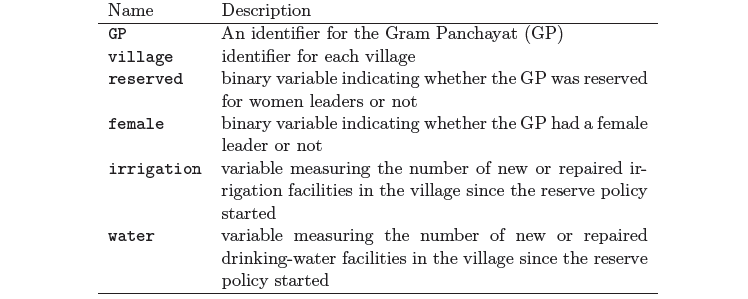
\includegraphics[width=0.7\linewidth]{women_desc}
\end{figure}


\newpage
\begin{enumerate}
	\item [(a)] State a null and alternative (two-tailed) hypothesis.
	\subsection*{Answer:} 
	Null hypothesis: The reservation policy has no affect of the number of new or repaired drinking water facilities in the villages.
	\vspace{0.2cm}
	
	H0: $\beta$ = 0
	
	Alternative hypothesis: The reservation policy has an affect on the number of new or repaired drinking water facilities in the villages.
	\vspace{0.2cm}
	
	Ha = $\beta$ $\neq$ 0
	
	
	Where in both cases $\beta$ (the slope) is equal to the strength of association between a village having a female politician as a consequence of the reservation policy (i.e. the reservation policy) and the number of new or repaired drinking water facilities.
	\vspace{0.5cm}
	
	The independent (predictor/explanatory) variable in this case is whether or not a village has a women politician as a result of the reservation policy, the dependent (outcome/criterion) variable is the number of new or repaired drinking water facilities.
	\vspace{1cm}
	\item [(b)] Run a bivariate regression to test this hypothesis in \texttt{R} (include your code!).
	
	\subsection*{Answer:}
	To run a bivariate regression analysis a linear model can be created in R with the lm function.
	\begin{Verbatim}
#Fitting a linear model, water facilities against reservation policy.
		
model1 <- lm(water ~ reserved, data=west_bengal_data)
summary(model1)
		
#confidence interval (CI) for the slope (beta) of reservation policy.
#Beta(hat) +or- (t-score*SE)

confint(model1, "reserved", level=0.95)

9.252+(1.97*3.948)
9.252-(1.97*3.948)

#95% CI = (1.47444, 17.02956)
		
#Export model1 as LaTex code.
stargazer(model1)
	\end{Verbatim}
		\begin{table}[!htbp] \centering 
		\caption{Table of lm model1} 
		\label{} 
		\begin{tabular}{@{\extracolsep{5pt}}lc} 
			\\[-1.8ex]\hline 
			\hline \\[-1.8ex] 
			& \multicolumn{1}{c}{\textit{Dependent variable:}} \\ 
			\cline{2-2} 
			\\[-1.8ex] & water \\ 
			\hline \\[-1.8ex] 
			reserved & 9.252$^{**}$ \\ 
			& (3.948) \\ 
			& \\ 
			Constant & 14.738$^{***}$ \\ 
			& (2.286) \\ 
			& \\ 
			\hline \\[-1.8ex] 
			Observations & 322 \\ 
			R$^{2}$ & 0.017 \\ 
			Adjusted R$^{2}$ & 0.014 \\ 
			Residual Std. Error & 33.446 (df = 320) \\ 
			F Statistic & 5.493$^{**}$ (df = 1; 320) \\ 
			\hline 
			\hline \\[-1.8ex] 
			\textit{Note:}  & \multicolumn{1}{r}{$^{*}$p$<$0.1; $^{**}$p$<$0.05; $^{***}$p$<$0.01} \\ 
		\end{tabular} 
	\end{table} 
Using the stargazer package in R, the above table can be exported into LaTex from the linear model produced by the lm function in R.

There is a positive association between a village having the reservation policy and the number of new or repaired drinking water facilities.
In villages with the reservation policy there are as few as 1.47444 more new or repaired drinking water facilities, and as many as 17.02956 more new or repaired drinking water facilities, when compared to villages without the reservation policy.

Because the confidence interval does not include a value equal to or less than zero, we have sufficient evidence to reject the null hypothesis, and consider the alternative hypothesis to be true.

\textbf{At the 95 percent confidence interval we have sufficient evidence to reject the null hypothesis.}

The positive association can be seen on the following scatter-plot.
\begin{center}
	\includegraphics{"Reservation policy ~ water facilities (ggplot2)"}
\end{center}

	


	\vspace{6cm}
	\item [(c)] Interpret the coefficient estimate for reservation policy.
	\subsection*{Answer:}
	
		Because the independent variable in this case is a binary/categorical variable. 
	\begin{Verbatim}
#The predicted value of Y(hat) is equal to alpha (intercept) plus beta (slope) 
multiplied by the state of the binary independent (dummy) variable (0 or 1).
		
#Model for reservation policy.
14.738+(9.252*1)
#Model for villages without the reservation policy.
14.738+(9.252*0)
	\end{Verbatim}
	This tells us that the predicted average of number of new or repaired drinking water facilities in villages with the reservation policy is 23.99, and the predicted average number of new or repaired drinking water facilities in villages without the reservation policy is 14.738. 
	
	The coefficient estimate for reservation policy is +9.252, which means that on average  villages with the reservation policy had 9.252 more new or repaired drinking water facilities than villages that did not have the reservation policy, with a standard error of 3.948. 
	
	The p-value also suggests statistically significant results, as indicted in the bottom of table 1 "lm of model1". The p-value is calculated in R as 0.0197 for the linear model, which given $\alpha$ = 0.05 at the 95 percent confidence interval suggests statistically significant results. 
	
	\section*{Biblography:}
	\begin{itemize}
		\item Simple Linear Regression - One Binary Categorical Independent Variable | Practical Applications of Statistics in the Social Sciences | University of Southampton (no date). Available at: \href{https://www.southampton.ac.uk/passs/confidence_in_the_police/multivariate_analysis/linear_regression.page}{link} (Accessed: 14 October 2023).
		
		\item Simple Linear Regression with a Binary Explanatory Variable (2020). Available at: \href{https://www.youtube.com/watch?v=53lhpwa3rwY}{link} (Accessed: 14 October 2023).
		\item Dr. Jeffery Ziegler's lecture slides.
		\item Hannah Frank's tutorial material.
		\item Learn Statistical Regression in 40 mins! My best video ever. Legit. (2023). Available at: \href{https://www.youtube.com/watch?v=eYTumjgE2IY}{link} (Accessed: 15 October 2023).
		\item t-Tables (no date). Available at: \href{https://faculty.washington.edu/heagerty/Books/Biostatistics/TABLES/t-Tables/}{link} (Accessed: 15 October 2023).
		\item ‘Use of Tilde ~ in R’ (2021) GeeksforGeeks, 25 November. Available at: \href{https://www.geeksforgeeks.org/use-of-tilde-in-r/}{link} (Accessed: 15 October 2023).
		
		
		
		
		
	\end{itemize}

		
\end{enumerate}

\end{document}
